\begin{filecontents*}{example.eps}
gsave
newpath
  20 20 moveto
  20 220 lineto
  220 220 lineto
  220 20 lineto
closepath
2 setlinewidth
gsave
  .4 setgray fill
grestore
stroke
grestore
\end{filecontents*}

\RequirePackage{fix-cm}
\documentclass{svjour3}                     % onecolumn (standard format)
\smartqed  % flush right qed marks, e.g. at end of proof
\usepackage{graphicx}
%\usepackage{mathptmx}      % use Times fonts if available on your TeX system


% insert here the call for the packages your document requires
\usepackage{natbib}
\usepackage{csvsimple}
\usepackage{breakcites}
\usepackage{caption}
\usepackage{blindtext}
\usepackage{amsmath}
\usepackage{float}
\usepackage{graphicx}
\usepackage{geometry}
\usepackage{longtable,array}
\usepackage{subfig}
\usepackage{graphicx}
\usepackage{url}
\usepackage{pdflscape}

\begin{document}
\title{x}
\date{}
\subtitle{x}
\titlerunning{x}        
\author{Matt Larriva, CFA         \and
        Peter Linneman, PhD.
}

%\authorrunning{Short form of author list} % if too long for running head

%\institute{M. Larriva\at
%              \email{mlarriva@fcpdc.com}           %  \\
%             \emph{Present address:} of F. Author  %  if needed
%           \and
%           P. Linneman\at
%              \email{plinneman@linnemanassociates.com} %  \\ 
%}

%\date{Received: date / Accepted: date}
% The correct dates will be entered by the editor

\maketitle

\begin{abstract}

\subsection*{Purpose}
To explain both national and market-level cap rate changes as simply an interaction between Gross Domestic Product and Consumer Price Index.

\subsection*{Design/Methodology/Approach}
We use a binary logistic regression with binary independent variables, trained on a synthetic minority over-sampling set, to explain cap rate expansion and contraction at the national level and at 20 MSAs.

\subsection*{Results}
Both the national model and the MSA models capture around 40\% of all cap rate expansion periods with a robust confusion matrix.

\subsection*{Originality}
This model contributes to the existing corpus by 1) establishing a statistically significant relationship between GDP, CPI, and cap rates which 2) holds explanatory power at the national and MSA levels, by 3) mapping the ground truth from scalar to binary.

\subsection*{Practical Implications}
The accuracy of the model suggests a simpler and more robust explanation for understanding cap rates and navigating property markets in an environment of fluctuating interest rates. 


\keywords{Binary Logistic Regression \and Cap Rates \and US Real Estate Markets \and Multifamily Cap Rate \and United States \and Apartment Cap Rate}

\end{abstract}

\pagebreak
\setlength{\parindent}{4em}
\setlength{\parskip}{1em}

\section{Introduction}
There is a clear desire in academic and professional circles to find a good predictor of cap rates to be able maximize potential returns. Despite the plethora of research attempting to establish the determinants of cap rates there exists a persistent degree of uncertainty in predicting cap rates. In fact, Liang Peng in ”Finding Cap Rates: A Property Level Analysis of Commercial Real Estate Pricing” found a strong positive relationship between pricing and risk for all property types. In other words the higher the cap rate the more uncertainty (Peng, 2013). Keeping in mind Peng’s findings macroeconomic variables may also contribute to uncertainty in the value of real estate assets. Fundamental macroeconomic variables such as inflation, deflation, and GDP growth despite their potential influence on uncertainty still appear to be the most promising variables for predicting future cap rates.

\label{intro}


\section{Literature Review}

The literature on cap rate forecasting is extensive, and it can be viewed well through two different lenses. The first framework is illustrated in Ghysels et. al. Forecasting Real Estate Prices \citep*{ghysels_plazzi_valkanov_torous_2013} which divides the literature by variable selection. The authors enumerate three camps: those models which use lagged return (or price change) as a variable, those which use ratios such as rent-to-price or price-to-income, and those which use more granular property or regional data. 

The second lens by which to view the research is through methodology selection, as documented by Larriva and Linneman \citep*{larriva2021determinants}. The authors divide the research into simple time series methods, multivariate timeseries, and machine learning methods. The division is roughly chronological. 

Neither lens quite suits this study's purpose, as the variables used in this work--raw GDP and CPI--are not often found in the research. More common is a spread to an inflation metric or a derivative of GDP. Separately, the level of granularity we seek to explain is somewhat uncommon (MSA level). More common is either property-level or national. Finally, the method we use is new to the research, to our review. The following section, then will seek to outline research that contains either GDP or inflationary metrics, or their derivatives, regardless of method or granularity.

In the mid-1990s, research was concentrated on either single-variate autoregressive methods \citep*{gau_1984}, \citep*{gau_1985}, \citep*{linneman_1986} or variations on OLS that used multi-stage estimation \citep*{case_shiller_1990}, \citep*{abraham_hendershott_1994}. The variables used in these methods of forecasting tended to fall into classes that line up with the components of a cap rate: risk-free rate, real interest rates, relative return expectations, and risk. Many models’ variables included a government long bond  to capture the risk-free and real rates, an economic spread (credit or pricing-based) to capture the relative expense or return of real estate, and macroeconomic factors to capture the  growth prospects and risk in the marketplace. Some models included a term to capture forward estimates including either sentiment or expected rent or NOI growth. This lines up with the Gordon growth model of pricing cap rates as the discount rate less the perpetual NOI growth rate. Thus, the value of macroeconomic factors, or their derivatives, was established.

\subsection{The Relationship between Inflation and Cap Rates}

Inflation has long been researched with regard to cap rates \citep*{froland1987determines}; \citep*{sivitanides2001determinants}; \citep*{chandrashekaran2000predictability}. Supporters suggest that inflation rates are inversely related to cap rates either via real rates, the weighted average  cost of capital, or increased borrowing costs. While there are myriad reasons why the relationship should hold, there are just as many observable exceptions--cases when cap rates increase when interest rates decline, or the reverse. Understandably then, the research into the topic reaches mixed conclusions.

\subsubsection{In Support of the Interest Rate and Cap Rate Relationship}
Froland \citep*{froland1987determines} reports negative correlations between cap rates and inflationary expectations. Sivitanides et. al. \citep*{sivitanides2001determinants} further supported and quantified this relationship at the MSA level. The authors use the average cap rates over the past 16 years of four property types across 14 metropolitan markets to examine how cap rates behave. And the statistical specification was estimated using a dual Time-Series Cross-Section method which corrects for cross section correlations and group-wise heteroskedasticity. Inflation was found to be a major driver of cap rates. In fact, Sivitanides et al. found that an expected increase in economy wide inflation of one percent annually lowers office cap rates by 46 basis points, multi-family cap rates by 40 basis points, retail cap rates by 54 basis points, and by 20 basis points in industrial cap rates.

Research from Wheaton et. al. \citep*{wheaton2001real} further substantiates the above work using a VAR model to show that inflation is a significant variable in determining cap rates at the MSA level. 

\subsubsection{In Opposition of the Interest Rate and Cap Rate Relationship}
In contrast to the above works, Chandrashekaran and Young \citep*{chandrashekaran2000predictability} find that there is not a statistically significant relationship between inflation and cap rates. To reach this conclusion Chandrashekaran and Young use two regression models: one with macroeconomic variables and one with lagged cap rates. The model with lagged cap rates uniformly performed better. The authors concluded that their attempt to predict cap rates using macroeconomic variables, such as inflation, were unsuccessful. 

Gimpelevich \citep*{Gimpelevich2011} supports Chandrashekaran and Young using Monte Carlo simulations of real estate returns called the Simulation-Based Excess Return Model (SERM). The simulation results in poor correlation between inflation rates and cap rates (Gimpelevich, 2011).

More recently, Larriva and Linneman \citep*{larriva2021determinants} used multivariate timeseries analysis to show the superiority of a model which did not use return expectations or inflationary metrics. Their model used granger causality to select variables and establish a highly robust explanatory and predictive VECM model, without the use of interest rates.

Although there are exceptions, different conclusions in this space can often be attributed to differences in data and methodology. Research which finds that inflation is a good predictor of future cap rates typically use time series data for both macroeconomic variables and cap rates while research which dismisses the value of inflation rates, generally, use cross sectional econometric methods.

We propose herein that perhaps the reason for the disagreement in the impact of inflation rates to cap rates is because only some models are including the vital second part of the relationship: GDP.


\subsection{GDP}

The growth or contraction of a nation or MSA's gross domestic product is likely the single most important indicator of economic health. That cap rates would be closely related to this metric is not surprising. And there is ample research which substantiates and explores this.

Granger causality between GDP and real estate markets was established in 1997 by Green \citep{green1997follow} who found that, under a wide variety of time series specifications, residential investment causes GDP, while non-residential investment is caused by GDP. The phrase "caused by" is used in the Granger sense in this context. 

Quan and Titman \citep{quan1997commercial} build on the Granger causality and seek to quantify the relationship. The team utilized time series regressions to examine the effects of changes in macroeconomic variables (including GDP) on real estate values and rents. To begin Quan and Titman explore the connection between stock and real estate market returns, and after establishing their connection the duo explore factors and develop regressions to explain this connection. The first theory they explore is that real estate and stock prices are both guided by future macroeconomic expectations such as GDP growth. The second is that commercial real estate prices rise and fall because of changing political and economic fundamentals, and under this theory the relationship between the stock and real estate market will be much weaker. After controlling for macroeconomic variance Quan and Titman find that the correlation between real estate and stock prices are primarily because of economic fundamentals, and that rental rates are strongly correlated with GDP growth.

Once this connection was established, research turned to its implication on an international scale: does worldwide GDP growth or local GDP growth have a larger effect on property values and cap rates? Case, et. al. \citep*{case2000global} explore whether or not correlations across global real estate markets are due to world changes in GDP, and estimate the value of local economic performance in real estate markets. This is an important question in real estate because all real estate is essentially local. And if local growth has a stronger effect on property values than national or global growth investors can better leverage local growth patterns to maximize return. The researchers found that that international property returns move together in dramatic fashion due to the effects of changes in GNP. Specifically, correlations of real estate are due in part to common exposure to fluctuations in the global economy, as measured by an equal-weighted index of international GDP changes. Some markets, such as Asia, are more effected by lo cal changes rather than world changes in GDP. In other words, even though real estate is fundamentally local changes in the global economy carry enough weight to have significant effects in local real estate markets.

\subsection{GDP and Inflation together}

Studies that focus on macroeconomic variables often include both GDP (or its derivative) and Inflation (or its derivative). The results often suggest that one variable is significant while the other is not. 

The aforementioned Quan and Titman research used cross sectional analyses to show that changes in GDP are very strongly related to movements in real estate values. But despite the significance of GDP, inflation and interest rates had relatively little effect on real estate values. Approaching the question with a timeseries analysis coroborated this conclusion. Quan and Titman found real estate values and rents were still significantly affected by changes in GDP. Inflation, again, appeared to be not significant. 

Aizenman and Jinjarak make a somewhat contrary finding. In their 2009 work, \citep*{aizenman2009current} they determine that the most economically significant variable in accounting for changes in real estate valuation is lagged real estate valuation appreciation (defined as real estate inflation minus CPI inflation), followed in importance by lagged declines of Current Account divided by GDP. Thus they note that an inflation derivative is more important than a GDP derivative. 

\subsection{Similar Models and Novelty}

The study that is most comparable to our own is that of Duca and Ling \citep*{duca2017taxes} whose research finds that cap rates are positively correlated with inflation via risk premia, and negatively correlated with rent growth expectations via GDP. Specifically, risk premia and real Treasury rates drive cap rates. They explain this theoretically via the discount factor (i.e. required rate of return).

Upon review, we note the frequency with which research disagrees on the significance (ordinal or absolute) of GDP metrics and inflation metrics. Our work makes three significant contributions to the existing body of work. 

First, we assert that neither GDP nor inflation variables are sufficient alone to explain cap rates. This can be seen by the above review. Simply using both as independent variables is not sufficient either. It is their interaction, we assert, that explains the most about cap rate directions. 

Second, we posit that we can learn more about cap rate determinants if we view cap rates as binary instead of continuous. While, of course, cap rate moves are non-discrete, this is not an useful way to analyse them, as real estate is still highly illiquid. The relevant question then, is not "will cap rates increase by, say,  0.0125 next year?" but instead "will cap rates increase next year?" Thus we model cap rate moves as random variables generated by a Bernouilli distribution as opposed to random variables generated by, say the Normal distribution. 

Finally, we propose a model that functions at the MSA and the national level. The more significant of these two is the former, because it determines the later. But the fact that the same data series are available at the nation and MSA and that they both corroborate the statistical findings is further attestation to the validity of the model.

\section{Data}
For the national model there are three data series that are used: the Consumer Price Index, the Gross Domestic Product, and the nominal Apartment cap rate series. 

The Gross Domestic Product is a quarterly, unadjusted (not de-seasoned) series from the St. Louis Fed's economic data page (FRED). It is important to use a nominal (versus real) series, as we are comparing this to the consumer price index, which is a close proxy to the interest rate series used to convert the GDP from nominal to real. That is to say, we would be double counting the impact of inflation.

The Consumer Price Index series is sourced to the Bureau of Labor Statistics, and it is also a non-seasonally adjusted series. In both cases, we did not seek to alter the series with seasonal adjustments because the raw data itself contains information which we do not wish to strip. Knowing if the economy grew faster than inflation, even if it was in 4Q, and even if it was due to holiday sales, is valuable information. Such a situation suggests a very different environment from its seasonally adjusted counterpart which may shows an economy in which 4Q growth is similar to say the prior quarter.

Finally, cap rate series at the national level are sourced to Green Street. Green Street defines its cap rate series as the next-twelve-months' NOI divided by the spot asset value. 

MSA-level data follows the conventions of the national data. Non-seasonally adjusted series are selected both for MSA GDP and the MSA's CPI. The former is from FRED while the later is from the Bureau of Labor Statistics.

As national CPI is presented monthly, and national GDP is presented quarterly, we proceded with quarterly data for the national model, pairing the CPI release most close to the GDP release. 

More challenging was the MSA-level data wherein GDP is presented only annually and CPI is presented with varying frequencies depending on the region. Atlanta is published on even months. Boston is published on odd months, and New York is published monthly. Some are bimonthly. The Bureau of Labor statistics only offers CPI measures for 22 Core Based Statistical Areas. Two of these are "Urban Alaska" and "Urban Hawaii", but these have no equivalent GDP series, so they were discarded. The remaining 20 CBSAs have GDP series. But the GDP series are not necessarily for the exact same areas i.e, some GDPs are published for an MSA, some are published for a CBSA. Adding to this confusion: the BLS revised its reporting in 2018 and started offering CBSA measurements instead of MSA measurements, thus revising the coverage areas.

We attempt to reconcile this by matching MSA to CBSA where needed (between the BLS and Fed). And we average the measurements of CPI over a year before matching them to the GDP metrics. In this way, we end up with 21 geographies: 20 CBSAs and 1 national geography. Each geography has a cap rate, CPI, and GDP. 

It is worth addressing the question, "is this simply 'real interest rates' by a different name?" It is not. Mathematically, the series have very low correlation. Practically, real rates contain an expectation of returns and an expectation of inflation, whereas GDP and CPI are merely spot empirical values.
 
\section{Model Construction}

\subsection{Model Selection}
While most analyses forecasting cap rates allow the random variable to be generated from a normal distribution, we opted instead to represent the variable as generated from a Bernoulli distribution. While this choice might be unorthodox--modeling a continuous variable like percentage as a binary variable-- we argue that it is well suited for two reasons. 

First, it is practical. Real estate is not an equity, it is an alternative asset. As such, it is illiquid. This lack of liquidity means an investor cannot enter and exit the market readily. As such, a would-be buyer is somewhat ambivalent between caring if a cap rate will go up by 40 basis points next year and if it  will simply go up. In either case, next year's prices will offer a better value. Similarly a would-be seller should be ambivalent between knowing if next year a cap rate will go up by 10 basis points or if it will go up by 100. In either situation, next year is a worse time to sell than this year.  Contrast this with an equities trader who can easily place stop-losses or 'level-in' to a position. Such a trader cares very much whether his holdings will increase 10\% next year, hence estimating liquid asset pricing is well suited by a continuous variable. But estimating illiquid asset pricing is, we argue, better done with a discrete variable. 

Second, it maps to the binary nature of the motivation of the model: will GDP growth (contraction) exceed CPI growth (contraction)? It matters less the exact amount one exceede or does not exceed the other. We argue that the question is simply: can a landlord pass on rising expenses to tenants or not? In the case where GDP is rising faster than inflation, we argue the tenants will be wealthier than the growth in expenses, and thus able to absorb higher rents, creating an asset worth more. Conversely, when inflation outpaces the growth of the economy, we argue the tenant is not in a position to absorb higher costs, leaving the landlord to bear them, creating an asset worth less. 

Thus a logistic regression with a single binary input lent itself well to our analysis, with cap rate expansion as the response variable, and GDP change $ > $  CPI change as the independent variable. 

\subsection{Model Specification}

We preprocessed the GDP and CPI series differently for the national versus MSA model because the national data was more frequent. In both cases, the preprocessing included differencing the series and then creating a simple trailing average. The goal in smoothing the series was to prevent an overly sensitive signal if, say, one period had inflation that quickly reversed. 

CPI and GDP percentage changes at $t_0$ were compared to trailing average historical percentage changes. A  signal was generated when 1) the $t_0$ GDP change was less than its trailing average changes and 2) the $t_0$ CPI change was greater than its trailing averages. The signal suggests cap rate expansion in the next period. 

The cap rate series were simply differenced and their sign taken to be a boolean variable such that cap rate expansion is TRUE and cap rate non-expansion (and contraction) is FALSE.

To establish the validity of the model for predictive power, we used a training and testing data set.

For the MSA model, we trained five separate models (Year = 2015, 2016....2020) which were specified using only data prior to that date. The each of the five models were used to predict the next years' (Years 2016-2021, 2017-2021,...2021) cap rate expansions and contractions based on the signal series outlined above. Each of these five models were specified as one--that is the data from each MSA was stacked into one matrix, absent the name of the MSA, and used to specify the model. The model then predicted the future values for each MSA based only on that MSA's historical data. Thus the same estimators were used to forecast the cap rate activity of the out-of-sample periods. Only the test data changed (was limited to only one MSA).

National models were created every two years from 2000, as data is both more frequent and longer lived than MSA-level data. 

Then, to establish the validity of the models for explanatory power, we trained both the MSA model and the national models using all time periods available (in-sample).

The ground truth of cap rate expansion does not present a balanced set, as cap rate compressions are far more frequent than cap rate expansions (roughly two to three times more years see compressions than expansions). We overcame the imbalance through a Synthetic Minority Over-sampling Technique as created by \citep*{SMOTE}. This balanced the frequency of cap rate expansions and contractions to prevent a the logistic regression from estimating all compressions (which would produce a low-variance high-bias estimator).

\subsection{Model Goodness of Fit}

In both the National and the MSA models, the logistic regressions displayed consistent coefficients, inline with our hypothesis. The coefficients had low standard errors relative  to the coefficients' magnitude, and the 2.5\% to 97.5\% bounds did not include zero in any case. 

Where a year is listed in the Split-Year column, the data was segmented into training and test sets. The training periods were all prior to the split year, and the test set was the split year through 2021. When "all-time" is listed under the Split-Year, the model was trained on all data and evaluated on all avalailable data. 

The columns, "Coef.", "Std.Err.", "Z", "$P>|z|$", and the 2.5\% to 97.5\% bounds are all populated with the parameters from the trained models using the training data. The columns to the right, "accuracy" through "specificity" are based on the test data. 

It is worth noting that the coefficient decreased consistently as time advances, suggesting that perhaps the signal is not as robust as it once was. However the standard error decreases correspondingly, producing a Z score which is as high as the earlier periods. Still, though the coefficient is decreasing more recently, all of the train/test models had higher coefficients for lower standard errors than did the models trained on all data. This could be due to the difficulty of trying to incorporate the GFC and the unorthodox interest rate behavior of the COVID-19 era. 

\subsubsection{National Model}
\csvautotabular{"C:/Users/matth/Documents/GitHub/inflation_cr_expansion/output/national_fit.csv"}

\subsubsection{Jointly Trained MSA Model}
\csvautotabular{"C:/Users/matth/Documents/GitHub/inflation_cr_expansion/output/msa_level_fit.csv"}

%\subsubsection{Individually Trained MSA Model}
%\csvautotabular{"C:/Users/matth/Documents/GitHub/inflation_cr_expansion/output/individual_msa_level_fit.csv"}

\section{Results}

Upon implementing the models, results were evaluated using a confusion matrix, as the period we are attempting to capture--cap rate expansion-- is far less frequent than cap rate contraction. 

Accuracy (TP+TN/(TP+FP+TN+FN)) can be understood as the portion of time the model correctly identified a cap rate expansion or contraction. At the national level,cap rate expansion has happened 29.5\% of quarters since 2000. The model then is more accurate than forecasting constant cap rate contraction, which would have yielded an accuracy of 70.5\%. This is not true at the MSA level, where cap rates have expanded 27\% of the time (compressed 73\% of the time) and the model yielded only 62\% accuracy. That is, it would have done better by forecasting constant cap rate compression (yielding an accuracy of 73\%.

Those subtleties are why we further examine precision, recall, and specificity. Precision (TP/(TP+FP)) is the ratio of correctly predicted positive observations to total predicted positive observations. The national model achieves 50\% precision, meaning half the time a signal is generated, it is accurate. The jointly trained MSA model has weak precision. 

Recall (TP/(TP+FN)) is the ratio of correctly identified cap rate expansions to the total number of cap rate expansions. In many MSAs there were only three or six years of cap rate expansions. Compare this to the national model which had far more quarters of cap rate expansion. The recall of the national model was high at 0.6, meaning 60\% of the times when cap rates expanded, the model correctly forecasted them. The recall of the MSA model was not particularly noteworthy.

The F1-score combines the precision and recall into their harmonic mean, and is valuable to consider percision and recall together, though it is less intuitive. 

Finally, the specificity (TN/(TN+FN)) of the national model was noteworthy, as it predicted cap rate compression with a higher accuracy than the true occurence of cap rate compression. MSA models were not successful in this regard. 

\subsubsection{National Model}
\csvautotabular{"C:/Users/matth/Documents/GitHub/inflation_cr_expansion/output/national_accuracy.csv"}

\subsubsection{Jointly Trained MSA Model}
\csvautotabular{"C:/Users/matth/Documents/GitHub/inflation_cr_expansion/output/msa_level_accuracy.csv"}


Still, despite the four metrics of the confusion matrix, there remains the question of efficacy in practice. Perhaps the model inadvertently only captured the smallest cap rate expansions and not the more pronounced one. Perhaps a buy-and-hold approach would have been better suited. 

To examine this we implemented the national and MSA models' recommendations and yielded the following results.

\begin{figure}
\hspace*{-0.25in}
\includegraphics{"C:/Users/matth/Documents/GitHub/inflation_cr_expansion/output/mas_graph_1_10.jpg"}
\end{figure}

\begin{figure}
\hspace*{-0.25in}
\includegraphics{"C:/Users/matth/Documents/GitHub/inflation_cr_expansion/output/mas_graph_11_20.jpg"}
\end{figure}

\begin{figure}
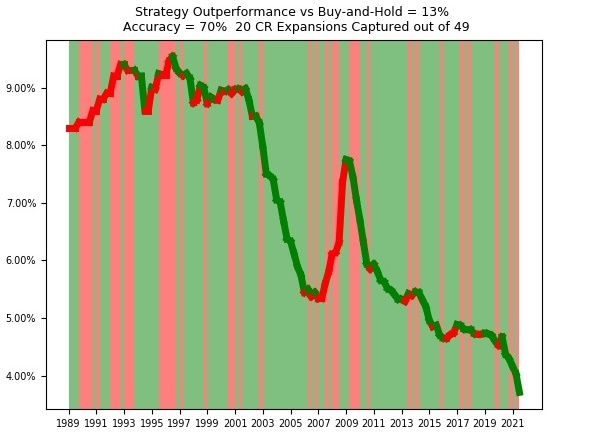
\includegraphics{"C:/Users/matth/Documents/GitHub/inflation_cr_expansion/output/national_performance.jpg"}
\end{figure}

Implementing the recommendations made by the model would have yileded cap rate compression 13\% greater than a buy-and-hold strategy. 

On average, implementing the MSA model resulted in significant outperformance relative to a buy-and-hold strategy. But the variance is quite high. 


\subsection{Analysis of Results}

The more robust predictor, in all cases, was the national model. This model, both in and out of sample, managed to forecast cap rate expansions accurately, with few false negatives and false positives. The model benefited from additional data points: both more history and more frequent readings. 

The MSA model that was jointly trained was relatively weak, which is likely owing to two factors. First, there is simply not enough data available. There were only 20 years of GDP and CPI data available consistently, and they were only reported annually. The model, however should not be disregarded, as data is becoming more widely distributed, with greater frequency, and with higher accuracy.

Upon further review, we noted that it seemed the MSAs wherein the model performed well were all established or low-population-growth cities, while the MSAs where the model performed poorly seemed to generally have higher population growth. 

%https://tableconvert.com/csv-to-latex
\begin{table}[!ht]
    \centering
    \begin{tabular}{|l|p{2cm}|p{2cm}|}
    \hline
        MSA & Outperformance vs Buy and Hold & HH Growth 2005 to 2020 \\ \hline
        Atlanta & 27\% & 21\% \\ \hline
        Baltimore & 66\% & 7\% \\ \hline
        Boston & 8\% & 11\% \\ \hline
        Chicago & -41\% & 5\% \\ \hline
        Dallas & -32\% & 29\% \\ \hline
        Denver & -51\% & 23\% \\ \hline
        Detroit & 62\% & -5\% \\ \hline
        Houston & -27\% & 34\% \\ \hline
        LosAngeles & 121\% & 3\% \\ \hline
        Miami & 196\% & 13\% \\ \hline
        Minneapolis & -22\% & 12\% \\ \hline
        NewYork & 87\% & 10\% \\ \hline
        Philadelphia & -26\% & 9\% \\ \hline
        Phoenix & 48\% & 22\% \\ \hline
        SanDiego & 21\% & 10\% \\ \hline
        SanFrancisco & 17\% & 9\% \\ \hline
        Seattle & -6\% & 24\% \\ \hline
        StLouis & 41\% & 6\% \\ \hline
        Tampa & 88\% & 7\% \\ \hline
        WashingtonDC & 3\% & 14\% \\ \hline
        Average & 29\% & 16\% \\ \hline
    \end{tabular}
\end{table}

Viewing these results in a regression, the results are more pronounced and show that household growth is significantly correlated with model underperformance, thus suggesting this model is very well suited for MSAs with national-average-like population growth. 

\begin{figure}
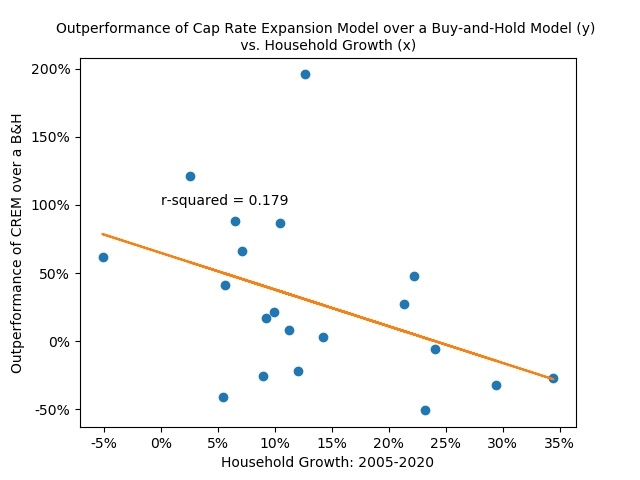
\includegraphics{"C:/Users/matth/Documents/GitHub/inflation_cr_expansion/output/msa_scatter.jpg"}
\end{figure}

Removing the leverage point (Miami 196\% outperformance and 13\% household growth) yields an even tighter relationship.

\begin{figure}
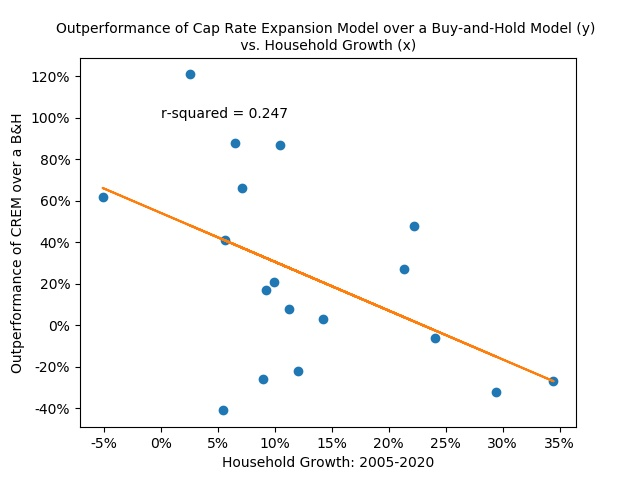
\includegraphics{"C:/Users/matth/Documents/GitHub/inflation_cr_expansion/output/msa_scatter_no_minmax.jpg"}
\end{figure}

And this makes intuitive sense: that a market with average-to-low organic growth would have its real estate values dictated by the interplay between inflation growth and GDP growth. Conversely, an area which was experiencing sharp population growth would have these dynamics overridden by the outsized demand for real estate.

\section{Conclusion}

\pagebreak


% Authors must disclose all relationships or interests that 
% could have direct or potential influence or impart bias on 
% the work: 
%
\section*{Declarations}
\subsection{Funding}
This research is a part of one author's role as VP of Research and Data Analytics at a Real Estate Private Equity firm. 

\subsection{Conflict of interest}
One author works for a Real Estate Private Equity firm which has ownership interest in many office and multifamily assets throughout the US. 

\subsection{Availability of data and material}
Data available upon request.

\subsection{Code availability}
Code available upon request.

\subsection{Authors' contributions}
Each of the authors confirms that this manuscript has not been previously published and is not currently under consideration by any other journal.


% BibTeX users please use one of
%\bibliographystyle{spbasic2}      % basic style, author-year citations
\bibliographystyle{apalike}
%\bibliographystyle{spmpsci}      % mathematics and physical sciences
%\bibliographystyle{spphys}       % APS-like style for physics
%\bibliography{}   % name your BibTeX data base

% Non-BibTeX users please use
%\begin{thebibliography}{}
%
% and use \bibitem to create references. Consult the Instructions
% for authors for reference list style.
%
%\bibitem{RefJ}
% Format for Journal Reference
%Author, Article title, Journal, Volume, page numbers (year)
% Format for books
%\bibitem{RefB}
%Author, Book title, page numbers. Publisher, place (year)
% etc
%\end{thebibliography}
\bibliography{bib} 

\end{document}
% end of file template.tex

